\section{Does It Hold Beyond One Checkpoint?}
\label{sec:generality}

Every new experiment above runs on Qwen2.5-14B-Instruct. That is a real exposure, and
not a generic one: \S\ref{sec:p1} shows a menu-signal effect \emph{reversing sign}
between $72$B and $14$B, so at least one interface effect in this literature is
model-specific. We therefore replicate the predicate contrast on two further families
chosen for independent pretraining rather than for scale.

\paragraph{Design.}
Llama-3.1-8B-Instruct and OLMo-2-1124-13B-Instruct, served under vLLM, against
Qwen2.5-14B as an anchor. Seeds, rounds, payoffs and prompts are identical across
models: the driver \emph{executes} the game module rather than reimplementing it, and
applies no chat template locally so that each model's own template is used
server-side. The comparison is therefore of models, not of prompt variants. Only the
text arms are run; the latent arm needs hidden states and cannot be served over an API.

\paragraph{Pipeline validation.}
The Qwen anchor runs the same seeds as \S\ref{sec:latent} through an entirely
different execution path---vLLM over HTTP rather than local \texttt{transformers}.
Bertrand reproduces to within $0.01$ on every quantity (no-channel $0.585\to0.580$,
proposal $0.450\to0.454$, contrast $-0.135\to-0.126$). IPD reproduces in direction and
is larger ($+0.400\to+0.700$) with overlapping intervals; lock-in is a binary outcome
at $n{=}20$ where the standard error is $\approx0.10$, so a $1.5$-SE gap is
unremarkable, but we report it as run-to-run variance rather than smooth over it.

\begin{table}[t]
\centering\small
\caption{\textbf{The market effect across three model families}, $20$ seeds per arm,
matched seeds and prompts. Bracketed values are bootstrap $95\%$ intervals. Pooling is
random-effects (DerSimonian--Laird): between-model variation is the quantity of
interest here, and a fixed-effects pool would treat it as noise.}
\label{tab:generality}
\begin{tabular}{lccc}
\toprule
model & no-channel $K$ & proposal $-$ none & proposal $-$ intention \\
\midrule
Qwen2.5-14B  & $0.580$ & $-0.126$ $[-0.203,-0.054]$ & $-0.111$ $[-0.181,-0.047]$ \\
Llama-3.1-8B & $0.827$ & $-0.041$ $[-0.061,-0.021]$ & $-0.031$ $[-0.054,-0.006]$ \\
OLMo-2-13B   & $0.650$ & $-0.075$ $[-0.125,-0.028]$ & $-0.058$ $[-0.119,-0.003]$ \\
\midrule
\textbf{pooled} & --- & $\mathbf{-0.069}$ $[-0.113,-0.026]$ & $\mathbf{-0.058}$ $[-0.103,-0.014]$ \\
\multicolumn{4}{l}{\footnotesize heterogeneity $I^2=65\%$ / $61\%$; all three same sign} \\
\bottomrule
\end{tabular}
\end{table}

\begin{figure}[t]
\centering
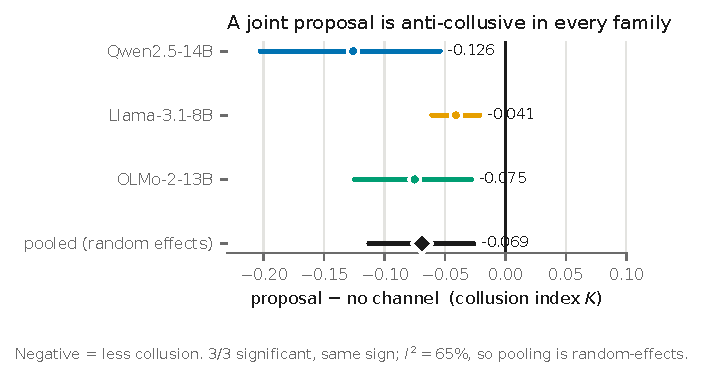
\includegraphics[width=0.72\textwidth]{figures/f5_generality.pdf}
\caption{\textbf{The market contrast on three independent model families.} Points are
per-model estimates with bootstrap $95\%$ intervals; the diamond is the random-effects
pool. All three fall left of zero. Heterogeneity is substantial ($I^2=65\%$) and is
reported rather than pooled away.}
\label{fig:generality}
\end{figure}

\paragraph{The market result replicates; the magnitude does not.}
A joint proposal is anti-collusive in all three families, three of three significant,
all the same sign (Table~\ref{tab:generality}). The pooled estimate is $-0.069$
$[-0.113,-0.026]$. Heterogeneity is substantial ($I^2=65\%$) and we do not smooth it
away: Llama's effect is a third of Qwen's, and the reason is visible in the same table.
Llama's no-channel baseline is $K=0.827$ against Qwen's $0.580$---it already prices
near joint monopoly before anyone speaks, leaving far less room to fall. Effect sizes
in this apparatus are bounded by headroom, which is itself model-specific.

\paragraph{The dilemma result is measurable in one family only.}
Neither Llama-3.1-8B nor OLMo-2-13B reaches cooperation lock-in under \emph{any} arm:
$0/60$ matches each, with mean cooperation $0.19$ and $0.18$. Those are capability
floors, not refutations, and we exclude them from pooling rather than counting them as
zeros---averaging a floor into a generality claim is a straightforward way to
manufacture a null. Qwen2.5-14B alone gives $+0.700$ $[+0.500,+0.900]$.

This is a genuine boundary on the IPD result and we state it as one. Cooperation
lock-in requires a model that can sustain cooperation at all, and two of the three
models we tested cannot. The claim that survives is conditional: \emph{where} a model
can coordinate, the predicate governs whether it does. Whether the smaller models fail
for capability reasons or because this particular scaffold is hostile to them is not
something these runs separate.

\paragraph{What the generality run does not cover.}
Three families, all $8$--$14$B, all instruction-tuned, all English. The prior work's
$72$B results are not re-run here, so the sign reversal reported in \S\ref{sec:p1}
remains uncalibrated against these models. And the latent channel of
\S\ref{sec:latent} is tested on one model only; nothing here speaks to whether a codec
built between two \emph{different} families transfers as cleanly.

% ======================================================================
